\documentclass[11pt]{article}
\usepackage{amsfonts, amssymb, amsmath}
\usepackage{xcolor}
\usepackage[a4paper,margin=1.5cm]{geometry}
\usepackage{array}
\usepackage{pgf}
\usepackage{pgfpages}
\usepackage{hyperref}
\usepackage{tcolorbox}
\usepackage{caption}
\usepackage{subcaption}
\usepackage{float}
\usepackage{tikz}
\usepackage{pgfplots}
\usepackage{enumitem}
\usepackage{fancyhdr}
\usepackage{background}
\usepackage{cancel}
\usetikzlibrary{calc}


\newcommand{\choice}[1]{\textbf{(#1)}}
%\newcommand{\tf}{(\CheckBox[bordercolor=]{T},\CheckBox[bordercolor=]{F})}
\def\DefaultOptionsofCheckBox{print,bordercolor=}

% Borderless Checkbox
\newcommand{\checknb}[1]{\CheckBox[bordercolor=, name=#1]{}}

% Blank(1.5cm)
\newcommand{\blank}[1]{\underline{\TextField[name=#1,align=1, bordercolor=, color=blue, width=2.5cm]{}}}

\newcommand{\cellfill}[1]{\TextField[name=#1, bordercolor=, width=0.7cm, height=0.5cm, align=1, color=blue]{}}

% True/False
\newcommand{\tf}[2]{[\CheckBox[name=#1 , bordercolor=]{True} ; \CheckBox[name=#2 , bordercolor=]{False} ]}

% Answer
\newcommand{\ansbox}[1]{\TextField[bordercolor=, name=#1, width=0.8\textwidth, color=blue]{}}

% Column Centre Align
\newcolumntype{P}[1]{>{\centering\arraybackslash}m{#1}}

\SetBgScale{1}
\SetBgAngle{0}
\SetBgColor{black}
\SetBgContents{

\begin{tikzpicture}[overlay,remember picture]
    \draw [xshift=0mm,line width=1.5pt]
        ($ (current page.north west) + (1cm,-1cm) $)
        rectangle
        ($ (current page.south east) + (-1cm,1cm) $);
\end{tikzpicture}
}


\begin{document}

\begin{figure}[H]
\begin{subfigure}[b]{0.4\textwidth}
\centering
\LARGE \underline{\textsc{Topic}}\\
\Large \textsc{(Sub-Topic)}\\
\vspace{4mm}
\end{subfigure}
\begin{subfigure}[b]{0.6\textwidth}
\begin{tcolorbox}
\begin{tabular}{lr}
Name \,: \underline{\TextField[bordercolor=, width=3.2cm, name = Name]{}} &\\
Grade : \underline{\TextField[bordercolor=, width=3.2cm, name = Grade]{}} &Date : \underline{\TextField[format   ={AFDate_FormatEx("dd.mm.yyyy");}, keystroke={AFDate_KeystrokeEx("dd.mm.yyyy");}, bordercolor=, width=3.2cm, name = Date]{}} \vspace{1mm}
\end{tabular}
\end{tcolorbox}
\end{subfigure}

\end{figure}

\hrule\vspace{1mm}
\hrule
%---------------------------------------------------
\begin{center}
\Large Practice Problems $-$ 1
\end{center}
\begin{enumerate}[label=\textbf{\arabic*)}]
\item[]The tables show input and output values of functions similar to $f(x)=ax$, Write the corresponding function for each table.
\item[\textbf{0)}] \begin{tabular}[t]{|P{1.5cm}||*{6}{P{6mm}|}}
\firsthline
$x$  & 1 & 2 & 3 & 4 & 5\\
\hline
$f(x)$ & 3 & 6 & 9 & 12 & 15\\
\hline
\end{tabular}\hspace{1cm}
$f(x)=\,\,${\TextField[readonly=true, bordercolor=, width=2.5cm]{$3x$}}\\

\item \begin{tabular}[t]{|P{1.5cm}||*{6}{P{6mm}|}}
\firsthline
$x$  & 54 & 42 & 24 & 18 & 72\\
\hline
$f(x)$ & 9 & 7 & 4 & 3 & 12\\
\hline
\end{tabular}\hspace{1cm}
$f(x)=\,\,$ \blank{q2a}\\

\item \begin{tabular}[t]{|P{1.5cm}||*{6}{P{6mm}|}}
\firsthline
$x$  & 2 & 4 & 8 & 16 & 32\\
\hline
$f(x)$ & 3 & 6 & 12 & 24 & 48\\
\hline
\end{tabular}\hspace{1cm}
$f(x)=\,\,$ \blank{q3a}\\

\item \begin{tabular}[t]{|P{1.5cm}||*{6}{P{6mm}|}}
\firsthline
$x$  & 8 & 5 & 12 & 11 & 102\\
\hline
$f(x)$ & 64 & 40 & 96 & 88 & 816\\
\hline
\end{tabular}\hspace{1cm}
$f(x)=\,$ \blank{q4a}\\\\


\item Identify the function for the given plot:
\begin{figure}[H]
	\centering
	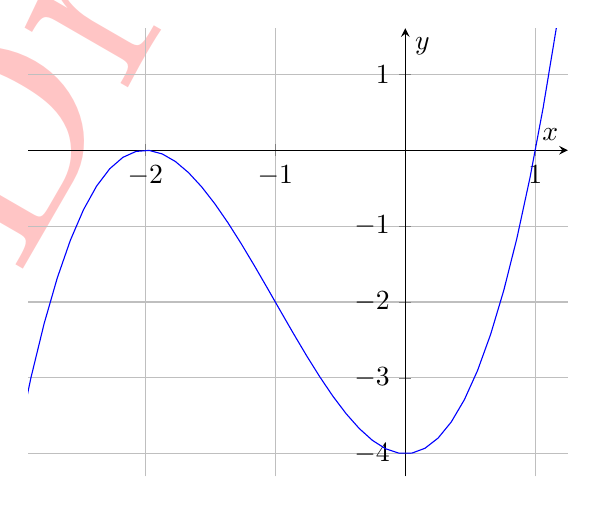
\begin{tikzpicture}
		\begin{axis}[samples=100, scale=1,
					xmin=-2.9,xmax=1.25,ymin=-4.3,
					grid=both, xlabel=$x$, ylabel=$y$,
					axis lines = middle,
					minor tick num=0]
		\addplot[blue]{(x-1)*(x+2)^2};
		\end{axis}
	\end{tikzpicture}
\end{figure}
\begin{tabular}{lll}
a)&$f(x)=x(x+2)(x-1)$ & - \checknb{4a} \\\\
b)&$f(x)=(x-1)(x+2)^2$ & - \checknb{4b}\\\\
c)&$f(x)=x(x-1)(x+2)^2$ & - \checknb{4c}\\\\
d)&$f(x)=(x-1)^2(x+1)^2$ & - \checknb{4d}\\\\
\end{tabular}\\\\

\newpage
\item Identify the plot of $y=x+2$
\begin{figure}[H]
	\begin{subfigure}[b]{0.5\textwidth}
	\centering
	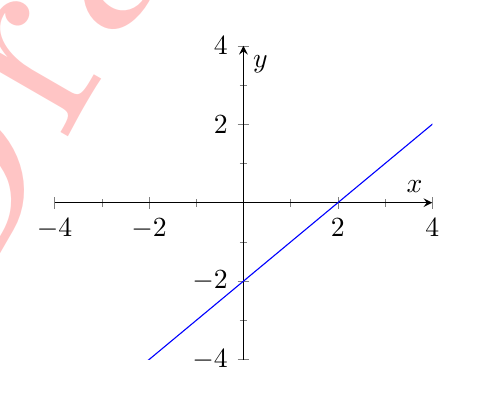
\begin{tikzpicture}
		\begin{axis}[scale=0.7,axis lines=middle,xmin=-4,xmax=4, ymin=-4,ymax=4,xlabel=$x$,ylabel={$y$}, grid=none, samples=100, minor tick num=1, minor grid style=dashed]
		\addplot[blue](x,x-2);
		\end{axis}
	\end{tikzpicture}
	\caption*{(a): \checknb{5a}}
	\end{subfigure}
	\begin{subfigure}[b]{0.5\textwidth}
	\centering
	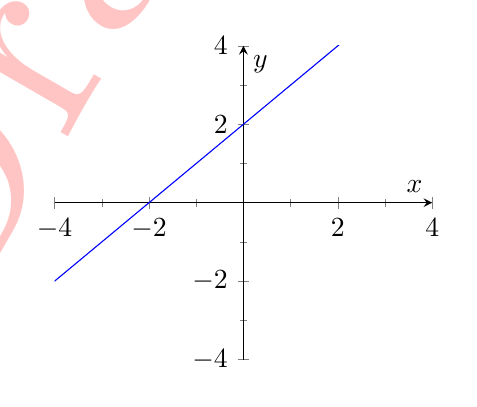
\begin{tikzpicture}
		\begin{axis}[scale=0.7,axis lines=middle,xmin=-4,xmax=4, ymin=-4,ymax=4,xlabel=$x$,ylabel={$y$}, grid=none, samples=100, minor tick num=1, minor grid style=dashed]
		\addplot[blue](x,x+2);
		\end{axis}
		\end{tikzpicture}
	\caption*{(b): \checknb{5b}}
	\end{subfigure}\vspace{0.5cm}
		\begin{subfigure}[b]{0.5\textwidth}
	\centering
	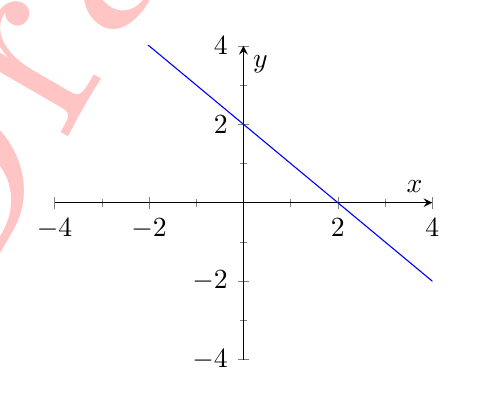
\begin{tikzpicture}
		\begin{axis}[scale=0.7,axis lines=middle,xmin=-4,xmax=4, ymin=-4,ymax=4,xlabel=$x$,ylabel={$y$}, grid=none, samples=100, minor tick num=1, minor grid style=dashed]
		\addplot[blue](x,-x+2);
		\end{axis}
	\end{tikzpicture}
	\caption*{(c): \checknb{5c}}
	\end{subfigure}
	\begin{subfigure}[b]{0.5\textwidth}
	\centering
	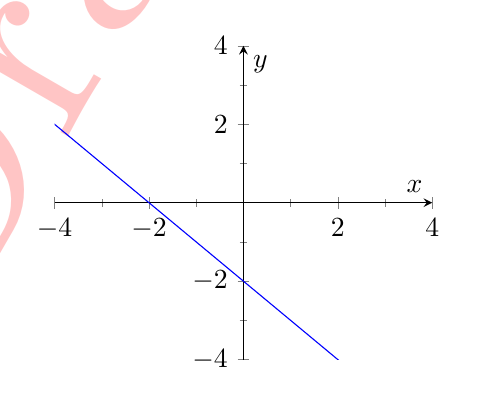
\begin{tikzpicture}
		\begin{axis}[scale=0.7,axis lines=middle,xmin=-4,xmax=4, ymin=-4,ymax=4,xlabel=$x$,ylabel={$y$}, grid=none, samples=100, minor tick num=1, minor grid style=dashed]
		\addplot[blue](x,-x-2);
		\end{axis}
	\end{tikzpicture}
	\caption*{(d): \checknb{5d}}
	\end{subfigure}
\end{figure}


\item Which of the following two plots describes the function $f(x)=2x+5$
\begin{figure}[H]
\begin{subfigure}{0.4\textwidth}
\centering
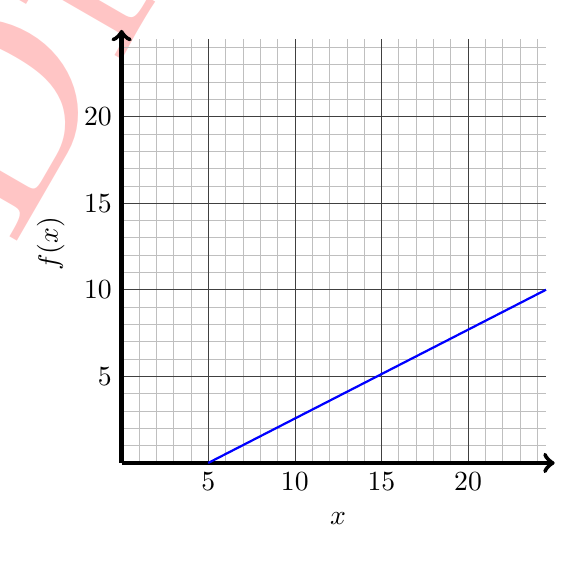
\begin{tikzpicture}[scale=1.1]
\draw [very thin, black!25!white](0,0) grid[step=.2cm] (4.9,4.9);
\draw [very thin, black!75!white](0,0) grid[step=1cm] (4.9,4.9);
\draw [ultra thick,->] (0,0) -- (0,5);
\draw [ultra thick,->] (0,0) -- (5,0);
\foreach \x in {5,10,15,20}
	\draw (\x/5,0) node[below] {\x};
\foreach \y in {5,10,15,20}
	\draw (0,\y/5) node[left] {\y};
\draw (0,2.5) node[above=0.5cm,left=0.9cm, rotate=90] {$f(x)$};
\draw (2.5,0) node[below=0.5cm] {$x$};

\draw [thick, blue] (1,0) -- (4.9,2);
\end{tikzpicture}
\caption*{(a): \checknb{q9a}}
\end{subfigure}
\begin{subfigure}{0.7\textwidth}
\centering
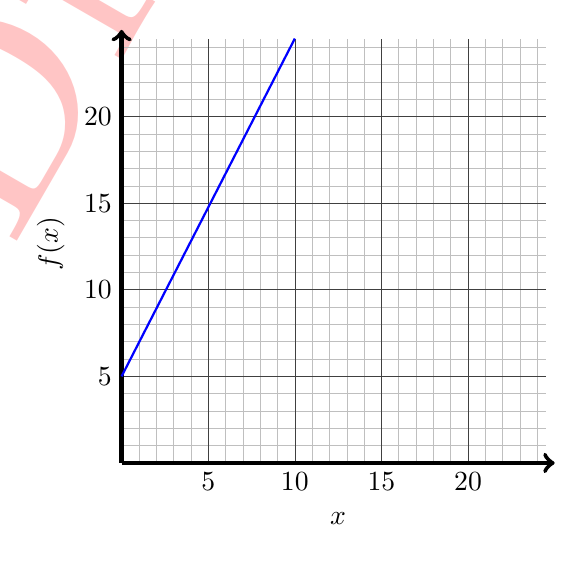
\begin{tikzpicture}[scale=1.1]
\draw [very thin, black!25!white](0,0) grid[step=.2cm] (4.9,4.9);
\draw [very thin, black!75!white](0,0) grid[step=1cm] (4.9,4.9);
\draw [ultra thick,->] (0,0) -- (0,5);
\draw [ultra thick,->] (0,0) -- (5,0);
\foreach \x in {5,10,15,20}
	\draw (\x/5,0) node[below] {\x};
\foreach \y in {5,10,15,20}
	\draw (0,\y/5) node[left] {\y};
\draw (0,2.5) node[above=0.5cm,left=0.9cm, rotate=90] {$f(x)$};
\draw (2.5,0) node[below=0.5cm] {$x$};

\draw [thick, blue] (0,1) -- (2,4.9);
\end{tikzpicture}
\caption*{(b): \checknb{q9b}}
\end{subfigure}
\end{figure}
\newpage

\item Write the complex numbers for all points given the figure.
\begin{figure}[H]
\centering
    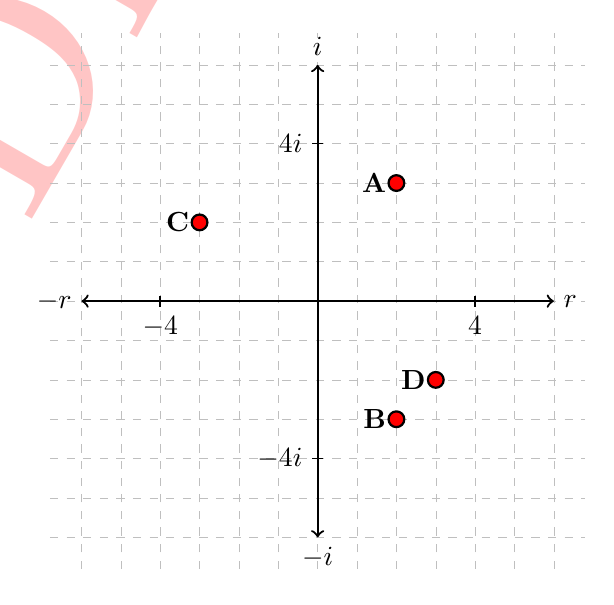
\begin{tikzpicture}
    % \fill [pink!50!white] (-3,-3) rectangle (3,3);
%    \draw[step=2cm,black,thin] (-2.9,-2.9) grid (2.9,2.9);
    \draw[step=.5cm,gray!50!white,very thin, dashed] (-3.4,-3.4) grid (3.4,3.4);
    \draw [thick, <->] (0,-3) -- (0,3);
    \draw [thick, <->] (-3,0) -- (3,0);
    \foreach \x in {-4,4}
	   \draw [thick](0.5*\x cm,2pt) -- (0.5*\x cm,-2pt) node[anchor=north] {$\x$};
	\foreach \y in {-4,4}
    	\draw (2pt,0.5*\y cm) -- (-2pt,0.5*\y cm) node[anchor=east] {$\y i$};
	\foreach \x/\y/\z in {2/-3/B,2/3/A,-3/2/C,3/-2/D}
	    	\draw [fill=red, thick] (0.5*\x,0.5*\y) circle (1mm) node[anchor= east] {\textbf{\z}};
%	    	\draw (0.5*\x, 0.5*\y) node[anchor=south] {$A$};
%	\draw [fill= blue,thick](1.5,+1) circle (1mm) node[anchor=east] {\textbf{P}};
%	\draw [blue,thick, ->] (0,0) -- (1.5,-1);
    \draw (0,3) node[anchor = south] {$i$};
    \draw (3,0) node[anchor = west] {$r$};
    \draw (0,-3) node[anchor = north] {$-i$};
    \draw (-3,0) node[anchor = east] {$-r$};
%    \draw [red, thick,dashed, ->] (0,0) -- (30:2cm);
%    \draw [red, thick, ->] (0,0) -- (120:2cm);
%	\draw [blue!100!black,thick,->,domain=30:120] plot ({0.5*cos(\x)}, {0.5*sin(\x)});
%    \draw [blue!100!black] (0.3,0.5) node[anchor=south] {$90^{\circ}$};
    \end{tikzpicture}
\end{figure}

\begin{tabular}{ll}
\textbf{A} :&\TextField[readonly=true,bordercolor=,]{$2 + 3i$} \\
\textbf{B} :&\blank{7b} \\
\textbf{C} :&\blank{7c} \\
\textbf{D} :&\blank{7d} \\\\
\end{tabular}\\\\

\item[] Complete the tables for each equation.
\item \hfill $f(x)=2x^2 - 3$\hfill\mbox{}\\
\mbox{}\hfill \begin{tabular}[t]{|m{1.5cm}||*{6}{P{6mm}|}}
\hline
$x$  & 1& 3& 4& 7& 9& 12\\
\hline
$f(x)$ & \cellfill{q13a} & \cellfill{q13b} & \cellfill{q13c} & \cellfill{q13d} & \cellfill{q13e} & \cellfill{q13f}\\
\hline
\end{tabular} \hfill \mbox{}


\item \hfill $9y=3x$ \hfill\mbox{}\\
\mbox{} \hfill \begin{tabular}[t]{|m{1.5cm}||*{6}{P{6mm}|}}
\hline 
$x$  & \cellfill{q14a}  & \cellfill{q14b}  & 15 & 27 & \cellfill{q14c}  & \cellfill{q14d}   \\
\hline
$y$ & 3 & 15 & \cellfill{q14e}   & \cellfill{q14f}   & 6 & 12  \\
\hline
\end{tabular} \hfill \mbox{}


\item \hfill $g(x)=\dfrac{1}{2}x+\dfrac{1}{2}x$ \hfill\mbox{}\\
\mbox{} \hfill \begin{tabular}[t]{|m{1.5cm}||*{6}{P{6mm}|}}
\hline
$x$  & \cellfill{q15a} & 12& 17& 8& \cellfill{q15b} & \cellfill{q15c} \\
\hline
$g(x)$ & 1& \cellfill{q15d} & \cellfill{q15e} & \cellfill{q15f} & 9& 12\\
\hline
\end{tabular} \hfill \mbox{}


\end{enumerate}



\end{document}